% !TEX root = ./cvl.tex
\section{Multi-scale filtering Problem}
\label{sec:background}

In the multi-scale filtering problem we select the subsets of the dataset that should be displayed on each scale of the generated map. Below we define the basic components of the problem, and informally define the associated optimization problem. 

\subsection{Geospatial records and weights}
\label{sec:records}

The dataset is assumed to consist of a set of \emph{geospatial records} that are drawn from a database table. Each record has a geometry, e.g.\ is a point, line segment, polygon --- or is a collection of simple geometric entities. Also, each geospatial record has relevant associated information, for example a city name, a hotel name or a description of an incident that took place at the given spatial location. Each record is assumed to have a unique ID.

Each record is assigned a \emph{user defined weight} using CVL (see Section~\ref{sec:cvl:language}). The weight represents the relative importance of a record in the generated map; an important (or highly ranked) record has a higher weight than a less important record. Any subset of records --- or all records for that matter --- may have the same weight. Therefore, the weights induce a partial order of the records.

\subsection{Zoom levels and map constraints}
\label{sec:zoomlevels}

The map should be generated on multiple scales, as specified by the user. Let the zoom-levels run from 1 (lowest scale) to $\mathcal{Z}$ (largest scale). On a given zoom level, the map is rendered at a certain pixel resolution. Thus, for a given zoom level, we know the distance in pixels between geospatial locations. This gives rise to two particularly important constraints when generating a map for the dataset at a given zoom level.

Firstly, the principle of constant information density~\cite{topfer1966principles} implies that the number of records that can be displayed in an area of a certain pixel size should be bounded. Assume that we divide the complete map into cells (or tiles) of, say, 256 x 256 pixels. The \emph{visibility} constraint~\cite{sarma2012fusiontables} states that each cell can contain at most $K$ visible records, where $K$ is a user defined parameter.

Secondly, records cannot be too close to each other in the map --- otherwise the user will not be able to interactively manipulate records in the map. The \emph{proximity} constraint states that every pair of visible records must be separated by at least $d$ pixels, where $d$ is a user defined parameter.

In addition to these constraints that must hold separately for each zoom level, the filtering of the records must be consistent across zoom levels. The \emph{zoom-consistency} constraint~\cite{sarma2012fusiontables} states that when a record is filtered out at a given scale, it should also be filtered out at all \emph{lower} scales. When a user zooms out on a map, records can only disappear --- not reappear.

Apart from the zoom-consistency constraint which must hold for any map, the visibility and proximity constraints are optional. The user chooses the set of constraints that must hold for a given map, and can even define new constraints using the CVL language, see Section~\ref{sec:cvl:language}.

\subsection{Conflict sets}
\label{sec:conflicts}

For a given zoom level, we model constraints such as visibility or proximity constraints using the notion of \emph{conflict sets}. A conflict set is a set of records that cannot all appear simultaneously at a given zoom level. 

For the visibility constraint, one conflict set is generated for each cell that contains more than $K$ records. For the proximity constraint, one conflict set is generated for each pair of records that is less than $d$ pixels apart. An example is shown in Figure~\ref{fig:proximity:conflict}. A record can be in several conflict sets, which is the case for point $p$ in the example.

\begin{figure}[htbp]
\begin{center}
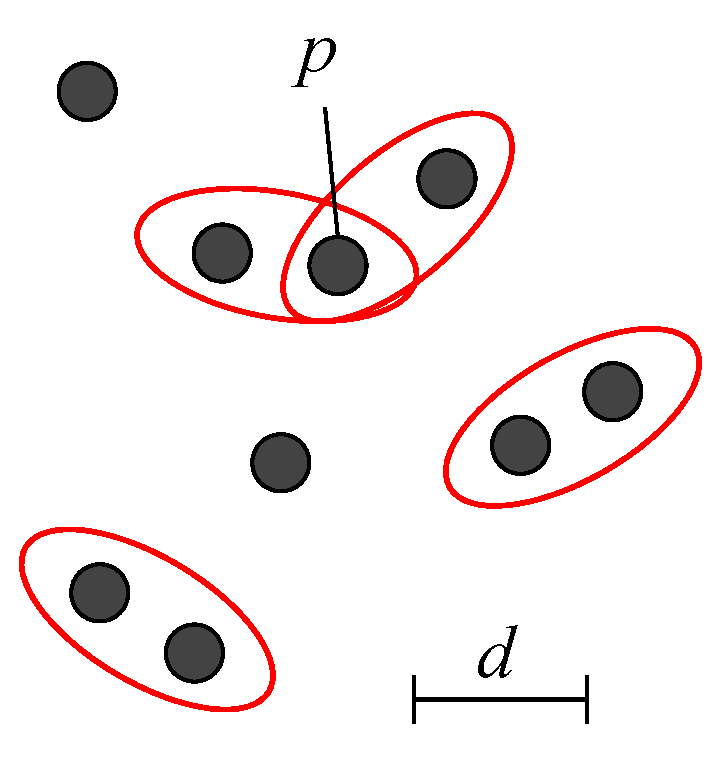
\includegraphics[scale=.3]{figs/cvl_proximity_conflicts.pdf}
\caption{Conflicts generated by the proximity constraint for distance $d$. Notice that point $p$ is a member of more than one conflict set.}
\label{fig:proximity:conflict}
\end{center}
\end{figure}

Any map constraint that can be formulated as a conflict set can be added by the user using CVL --- but this is also the only means of formulating general constraints at a given zoom level. 

Consider a conflict set containing $k_1$ records, where at most $k_2$ of these records can appear on the map (where $k_1 > k_2$). Then it is equivalent to state that at least $\lambda = k_1 - k_2$ of these records must be \emph{filtered out} at the given zoom level. In the mathematical formulation of the problem in Section~\ref{sec:optimizationmodel} we will use this alternative way to formulate conflict sets.

\subsection{Filtering as an optimization problem}
\label{sec:filtering}

The overall task of multi-scale filtering is to identify a subset of the dataset at each zoom-level, such that all constraints are satisfied, and such that the aggregate weight of records that are removed is minimized. Note that if a record is filtered out at, say, 7 zoom levels, then the record contributes to the aggregate weight 7 times its user defined weight (the record must necessarily be filtered out at the lowest 7 zoom levels due to the zoom-consistency constraint). In this manner, filtering out high-weight records at high zoom levels is particularly costly --- which is exactly what we would like to achieve. In Section~\ref{sec:optimizationmodel} we present a mathematical formulation of this optimization problem.
